\documentclass[11pt,oneside]{article}

\usepackage[T1]{fontenc}
\usepackage[utf8]{inputenc}
\usepackage{lmodern}
\usepackage{microtype}
\usepackage[a4paper,margin=26mm,headheight=14pt]{geometry}
\usepackage{amsmath,amssymb,amsthm,mathtools}
\usepackage{bm}
\usepackage{mathrsfs}
\usepackage{booktabs,longtable,tabularx,array,multirow}
\usepackage{graphicx}
\usepackage{caption}
\usepackage{placeins}
\usepackage{enumitem}
\usepackage{xcolor}
\usepackage{listings}
\usepackage{xurl}
\usepackage{hyperref}
\usepackage[nameinlink,capitalise,noabbrev]{cleveref}
\usepackage{fancyhdr}
\usepackage{setspace}

\hypersetup{
  colorlinks=true,
  linkcolor=blue!45!black,
  citecolor=blue!45!black,
  urlcolor=blue!55!black,
  pdftitle={Global Polynomial Interpolation of the Fabius and Rvachev Functions on Dyadic Combs},
  pdfauthor={OpenAI GPT-5.6 Pro}
}

\pagestyle{fancy}
\fancyhf{}
\lhead{Fabius--Rvachev interpolation on dyadic combs}
\rhead{Research report}
\cfoot{\thepage}

\newtheorem{theorem}{Theorem}[section]
\newtheorem{proposition}[theorem]{Proposition}
\newtheorem{lemma}[theorem]{Lemma}
\newtheorem{corollary}[theorem]{Corollary}
\newtheorem{conjecture}[theorem]{Conjecture}
\newtheorem{question}[theorem]{Research question}
\theoremstyle{definition}
\newtheorem{definition}[theorem]{Definition}
\newtheorem{experiment}[theorem]{Numerical observation}
\theoremstyle{remark}
\newtheorem{remark}[theorem]{Remark}

\newcommand{\R}{\mathbb R}
\newcommand{\N}{\mathbb N}
\newcommand{\Q}{\mathbb Q}
\newcommand{\Up}{\operatorname{up}}
\newcommand{\Fext}{\mathcal F}
\newcommand{\Lag}{\mathcal I}
\newcommand{\Leb}{\Lambda}
\newcommand{\dd}{\,\mathrm d}
\newcommand{\e}{\mathrm e}
\newcommand{\wt}{\operatorname{wt}}
\newcommand{\bigO}{\mathcal O}
\newcommand{\littleo}{o}
\newcommand{\norm}[1]{\left\lVert #1\right\rVert}
\newcommand{\abs}[1]{\left\lvert #1\right\rvert}
\newcommand{\floor}[1]{\left\lfloor #1\right\rfloor}
\newcommand{\ceil}[1]{\left\lceil #1\right\rceil}
\newcommand{\binomgen}[2]{\left(\!\!\binom{#1}{#2}\!\!\right)}
\newcommand{\statusproved}{\textsc{proved}}
\newcommand{\statusnumeric}{\textsc{numerical}}
\newcommand{\statusconj}{\textsc{conjectural}}

\lstset{
  basicstyle=\ttfamily\small,
  columns=fullflexible,
  breaklines=true,
  frame=single,
  showstringspaces=false,
  keywordstyle=\bfseries,
  commentstyle=\itshape
}

\title{\bfseries Global Polynomial Interpolation of the Fabius and Rvachev Functions on Dyadic Combs\\[4pt]
\large Exact arithmetic, Runge instability, endpoint-jet deflation, and frontier conjectures}
\author{Research report prepared with OpenAI GPT-5.6 Pro}
\date{28 August 2026}

\begin{document}
\maketitle

\begin{abstract}
The Fabius function is infinitely differentiable, exactly evaluable at dyadic rationals, symmetric about the midpoint, flat at both endpoints, and nowhere analytic on its active interval.  These properties make it a particularly sharp test case for global polynomial interpolation: the data are arithmetically ideal, while the analytic regularity is deliberately hostile to naive high-degree approximation.

This report studies the unique degree-$N$ Lagrange polynomial through the dyadic comb $j/N$, $0\le j\le N$, with $N=2^m$, and corresponding interpolants of Rvachev's compactly supported function $\Up$.  A recursive audit of the supplied repository separates this problem from two neighboring topics already present there: geometric-node Lagrange formulas used as coefficient extractors for $q$-series, and stable local dyadic reconstructions such as piecewise-linear/Faber--Schauder schemes.  The global additive-comb problem treated here is different.

The main structural result is an exact family of endpoint-Hermite interpolants.  Let $S_r(x)=I_x(r+1,r+1)$ be the symmetric beta-polynomial smoothstep and $W_r(x)=[x(1-x)]^{r+1}$.  Then
\[
 H_{N,r}(x)=S_r(x)+W_r(x)\,\Lag_{N-2}^{\circ}
 \left(\frac{F-S_r}{W_r}\right)(x)
\]
interpolates all $N+1$ dyadic values and fixes the first $r$ derivatives at each endpoint.  Ordinary Lagrange interpolation is exactly the case $r=0$.  The formula preserves rationality and midpoint symmetry, gives a factored error identity, and yields a natural weighted Lebesgue function.

Endpoint jets can postpone visible oscillation by many orders of magnitude, but they cannot remove the underlying instability.  We prove an exponential lower bound for the weighted Lebesgue constant for every fixed $r$, and a stronger two-regime theorem showing that \emph{no sequence} of endpoint orders $r=r_N$ makes this interpolation family stable: the best possible weighted operator norm remains exponential in $N$.  The two competing instability mechanisms predict
\[
 r_{\mathrm{bal}}(N)\sim \frac{N}{\log_2N-3/2},
\]
in close agreement with high-precision experiments.  Nevertheless, the optimized actual error falls to about $7.6\times10^{-7}$ at $(N,r)=(32,8)$, then rises to $4.0\times10^{-3}$ at $(128,23)$ and approximately $9.3\times10^8$ at $(256,40)$.  Matching derivatives at \emph{every} dyadic node is worse: matching only $F'$ already produces error about $1.5\times10^7$ at $N=32$.

Additional exact results include Newton-forward and barycentric forms, a $2$-adic valuation law for the dyadic-comb barycentric weights, an even-polynomial reduction for the full Rvachev comb, and a Lambert-$W$ saddle heuristic for the migration of the error peak.  The report distinguishes proved statements, numerical observations, and conjectures throughout, and ends with alternatives that retain dyadic data without inheriting global Runge instability.
\end{abstract}

\tableofcontents
\newpage

\section{Scope, corpus audit, and status of claims}
\label{sec:audit}

\subsection{What was read and what is new here}

The source corpus was audited recursively under
\begin{center}
\url{https://github.com/VladimirReshetnikov/ProveIt/tree/main/Analysis/FabiusFunction/docs}.
\end{center}
The audit used the live primary sources, the current consolidated ``non-formalized research frontiers'' volume, the draft manifest, the recursive inventory embedded in the corpus, and the archive indexes that identify renamed or superseded copies.  Historical duplicates were not counted as independent mathematical results.  The main current sources include:
\begin{itemize}[leftmargin=2em]
\item \path{Fabius_Function_and_Rvachev_Up/Fabius_Function_and_Rvachev_Up.tex};
\item \path{FabiusFunction_Mathematical_Glossary/FabiusFunction_Mathematical_Glossary.tex};
\item \path{Non_Elementarity_of_the_Fabius_Function/Non_Elementarity_of_the_Fabius_Function.tex};
\item \path{fabius_lean_walkthrough/fabius_lean_walkthrough.tex};
\item \path{non-formalized-research-frontiers/non-formalized-research-frontiers.tex};
\item consolidated draft families on inverse/sampling, representations, spectra/arithmetic, Thue--Morse, exponent and $q$-series methods, and integral transforms;
\item published-paper sources and archived historical lineages indexed under \path{papers/} and \path{archive/}.
\end{itemize}
The corpus's pinned recursive inventory records $67$ distinct \texttt{.tex} paths at one audit checkpoint; the live tree is more consolidated.  Full-text searches were made for \texttt{Lagrange}, \texttt{interpolation}, \texttt{Runge}, \texttt{Hermite}, \texttt{Lebesgue constant}, \texttt{equispaced}, and related variants.

Two adjacent bodies of work were found and deliberately not duplicated.
\begin{enumerate}[leftmargin=2em]
\item The frontiers volume uses Lagrange interpolation on \emph{geometric} nodes as an algebraic coefficient extractor for $q$-products and extrapolation.  Those formulas naturally produce $q$-binomial coefficients.
\item The representation and sampling material studies \emph{local} dyadic reconstruction, including piecewise-linear/Faber--Schauder and repeated-integration spline approximants with algebraic error bounds.
\end{enumerate}
The present report studies a single \emph{global} polynomial through the additive dyadic comb $j/2^m$, and confluent variants that impose derivatives.  No global Fabius/Rvachev Runge study or the beta-polynomial jet factorization below was found in the audited corpus.

\subsection{Evidence labels}

The report uses the following status convention.
\begin{center}
\begin{tabularx}{0.93\textwidth}{@{}p{0.19\textwidth}X@{}}
\toprule
Label & Meaning \\
\midrule
\statusproved & A complete argument is supplied here, or the statement is a direct specialization of a cited theorem. \\
\statusnumeric & Exact dyadic input data and high-precision evaluation support the claim, but no general proof is asserted. \\
\statusconj & A precise frontier statement suggested by theory and computation. \\
\bottomrule
\end{tabularx}
\end{center}
This distinction is essential.  Exponential growth of an interpolation operator does not by itself prove divergence on one particular function, while a spectacular numerical divergence does not by itself determine the exact asymptotic rate.

\section{Fabius and Rvachev background needed for interpolation}
\label{sec:background}

\subsection{Normalizations}

We use the conventions of the repository's primary exposition \cite{proveit-primary}.  The bounded Fabius function $F:\R\to[0,1]$ is $0$ on $(-\infty,0]$, $1$ on $[1,\infty)$, and satisfies on the active interval
\begin{equation}
 F'(x)=
 \begin{cases}
  2F(2x),&0\le x\le \tfrac12,\\
  2F(2-2x),&\tfrac12\le x\le1.
 \end{cases}
 \label{eq:F-dde}
\end{equation}
It obeys
\begin{equation}
 F(1-x)=1-F(x),\qquad F(1/2)=1/2,
 \label{eq:F-symmetry}
\end{equation}
and is flat at the endpoints:
\begin{equation}
 F^{(q)}(0)=F^{(q)}(1)=0\qquad(q\ge1).
 \label{eq:flatness}
\end{equation}
The even compactly supported Rvachev function is
\begin{equation}
 \Up(y)=F(1-|y|),\qquad |y|\le1,
 \label{eq:up-fold}
\end{equation}
with $\Up(y)=0$ for $|y|\ge1$.  In particular, $F(x)=\Up(x-1)$ on $[0,1]$.

The signed extension $\Fext$ satisfies $\Fext'(x)=2\Fext(2x)$ on all of $\R$.  The derivative tower proved in the repository gives
\begin{equation}
 \Fext^{(q)}(x)=2^{\binom{q+1}{2}}\Fext(2^q x),
 \qquad
 \norm{F^{(q)}}_{\infty}=2^{\binom{q+1}{2}}.
 \label{eq:derivative-tower}
\end{equation}
The norm is sharp.  Thus $F$ is $C^\infty$ but its derivative norms grow quadratically in the exponent.  This is one reason why the textbook remainder formula does not provide a useful convergence theorem for degree-$N$ interpolation.

\subsection{Exact dyadic values}

Arias de Reyna and Haugland developed exact arithmetic for dyadic values \cite{arias2018,haugland2016}; the repository packages it as a bit-recursive evaluator.  Let
\begin{equation}
 V_n=F(2^{-n}),\qquad V_0=1.
\end{equation}
One convenient recurrence is
\begin{equation}
 V_n=\frac{1}{(2^n-1)2^{\binom n2}}
 \sum_{k=0}^{n-1}\frac{2^{\binom k2}V_k}{(n-k+1)!}.
 \label{eq:V-recurrence}
\end{equation}
For $0<a<2^e$, write $b=\floor{\log_2a}$, $r=e-b$, $q=a-2^b$, and $y=q/2^e$.  Then
\begin{equation}
 F\!\left(\frac{a}{2^e}\right)
 =\sum_{j=0}^{r}\frac{2^{\binom{j+1}{2}}V_{r-j}}{j!}y^j
 -F\!\left(\frac{q}{2^e}\right).
 \label{eq:bit-split}
\end{equation}
Every value is rational.  Equations \eqref{eq:V-recurrence}--\eqref{eq:bit-split} are used in the supplied Python program, so numerical experiments do not import sampling error into the interpolation data.

\section{The global dyadic-comb Lagrange polynomial}
\label{sec:lagrange}

Fix
\begin{equation}
 N=2^m,
 \qquad x_j=\frac{j}{N},\quad 0\le j\le N,
 \qquad f_j=F(x_j).
 \label{eq:comb}
\end{equation}
Let $P_N$ be the unique polynomial of degree at most $N$ such that $P_N(x_j)=f_j$.

\subsection{Barycentric and Newton-forward forms}

For equispaced nodes, barycentric weights may be taken as
\begin{equation}
 \lambda_j=(-1)^j\binom Nj.
 \label{eq:full-bary-weights}
\end{equation}
Hence
\begin{equation}
 P_N(x)=
 \frac{\displaystyle\sum_{j=0}^{N}\frac{\lambda_j f_j}{x-x_j}}
 {\displaystyle\sum_{j=0}^{N}\frac{\lambda_j}{x-x_j}},
 \qquad x\notin\{x_0,\dots,x_N\}.
 \label{eq:bary-full}
\end{equation}
This is the second barycentric formula advocated by Berrut and Trefethen \cite{berrut-trefethen}.  It evaluates a fixed interpolation problem efficiently, but it does not repair the conditioning of equispaced polynomial interpolation.

Let $\Delta f_j=f_{j+1}-f_j$.  The Newton-forward form is
\begin{equation}
 P_N(x)=\sum_{k=0}^{N}\binom{Nx}{k}\Delta^k f_0.
 \label{eq:newton-forward}
\end{equation}
This identity is useful for exact symbolic work and links interpolation to the repository's finite-difference and binomial themes.

\begin{proposition}[Exact arithmetic and symmetry]
\label{prop:exact-symmetry}
For $N=2^m$, the polynomial $P_N$ has rational coefficients and satisfies
\begin{equation}
 P_N(1-x)=1-P_N(x).
 \label{eq:P-symmetry}
\end{equation}
Consequently $P_N(1/2)=1/2$, and every even derivative of $P_N(x)-1/2$ vanishes at $x=1/2$.
\end{proposition}

\begin{proof}
The nodes and data are rational, so the Vandermonde system has rational coefficients and a nonzero rational determinant.  For symmetry, the polynomial $1-P_N(1-x)$ has degree at most $N$ and, by \eqref{eq:F-symmetry}, takes the value $F(x_j)$ at every node.  Uniqueness gives \eqref{eq:P-symmetry}.
\end{proof}

\subsection{A dyadic $2$-adic law for the barycentric weights}

The real magnitudes of \eqref{eq:full-bary-weights} control Runge amplification, but the dyadic choice $N=2^m$ also gives an exact arithmetic stratification.

\begin{theorem}[$2$-adic valuation of the full-comb weights]
\label{thm:weight-valuation}
Let $N=2^m$.  For $1\le j\le N-1$,
\begin{equation}
 \nu_2\!\binom Nj=m-\nu_2(j).
 \label{eq:weight-valuation}
\end{equation}
\end{theorem}

\begin{proof}
Use
\[
 \binom Nj=\frac{N}{j}\binom{N-1}{j-1}.
\]
The binary expansion of $N-1=2^m-1$ consists entirely of ones.  Lucas's theorem implies that every coefficient in row $N-1$ is odd.  Taking $2$-adic valuations therefore gives \eqref{eq:weight-valuation}.
\end{proof}

This law is not visible in a generic equispaced grid.  It suggests a separate $2$-adic interpolation problem in which the same weights are arithmetically well structured even though they are disastrous in the real norm.  For the interior grid used later, the weights are $(-1)^{j-1}\binom{N-2}{j-1}$; Lucas's theorem shows that they are odd exactly when $j$ is odd, with higher valuations determined by binary carries.

\subsection{Why smoothness does not protect the interpolation}

The classical pointwise remainder has the form
\begin{equation}
 F(x)-P_N(x)=\frac{F^{(N+1)}(\xi_x)}{(N+1)!}
 \prod_{j=0}^{N}(x-x_j).
 \label{eq:remainder}
\end{equation}
For the Fabius function,
\begin{equation}
 \norm{F^{(N+1)}}_\infty=2^{\binom{N+2}{2}}.
\end{equation}
This factor overwhelms the elementary bounds on the nodal product, so \eqref{eq:remainder} does not imply convergence.  More conceptually, the equispaced Lebesgue constant grows exponentially; the classical Turetskii asymptotic is
\begin{equation}
 \Leb_N\sim \frac{2^{N+1}}{\e N\log N}.
 \label{eq:turetskii}
\end{equation}
See the surveys and analyses in \cite{brutman,smith-lebesgue,mills}.  The Coppersmith--Rivlin growth theorem gives a complementary description of how a polynomial can remain controlled at equispaced samples while becoming exponentially large between them \cite{coppersmith-rivlin}.  The impossibility theorem of Platte, Trefethen, and Kuijlaars places this phenomenon in a broader stability/convergence tradeoff for equispaced data \cite{platte-trefethen-kuijlaars}.

\section{Runge behavior of ordinary Fabius interpolation}
\label{sec:ordinary-runge}

\subsection{High-precision experiment}

The barycentric formula was evaluated with exact rational samples and $70$--$210$ decimal digits, depending on $N$.  Maxima were searched on a dyadic validation grid of spacing $2^{-13}$; symmetry reduced the search to $[0,1/2]$.  The reported Lebesgue constants are sampled on the same grid.

\begin{table}[htbp]
\centering
\caption{Ordinary global Lagrange interpolation on $j/N$.}
\label{tab:standard}
\small
\begin{tabular}{rrrrrr}
\toprule
$N$ & $\norm{F-P_N}_\infty$ & leftmost maximizer & $\min P_N$ & $\max P_N$ & $\Leb_N$ \\
\midrule
4   & $3.997\times10^{-2}$ & 0.092285 & $-3.94\times10^{-2}$ & 1.039 & $2.208$ \\
8   & $9.487\times10^{-3}$ & 0.040649 & 0 & 1 & $1.095\times10^{1}$ \\
16  & $3.797\times10^{-3}$ & 0.015381 & 0 & 1 & $9.345\times10^{2}$ \\
32  & $4.989$               & 0.007080 & $-4.989$ & 5.989 & $2.431\times10^{7}$ \\
64  & $3.590\times10^{7}$  & 0.003052 & $-3.590\times10^{7}$ & $3.590\times10^{7}$ & $4.405\times10^{16}$ \\
128 & $3.847\times10^{22}$ & 0.001343 & $-3.847\times10^{22}$ & $3.847\times10^{22}$ & $3.536\times10^{35}$ \\
\bottomrule
\end{tabular}
\end{table}

The error initially decreases, giving a misleading impression of convergence through $N=16$.  At $N=32$ a boundary oscillation dominates; by $N=128$ the interpolant is unusable over any ordinary floating-point scale.  The maximizer moves toward the endpoint roughly on the scale $1/N$.

\begin{figure}[htbp]
\centering
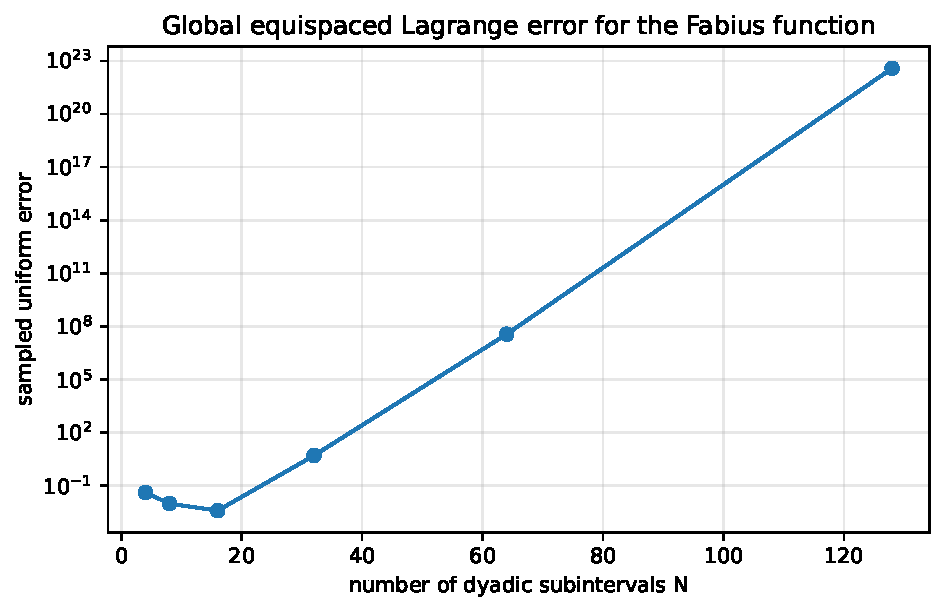
\includegraphics[width=0.82\textwidth]{figures/standard_error_growth.pdf}
\caption{Sampled uniform error of the ordinary dyadic-comb interpolant.  The transition between $N=16$ and $N=32$ is the visible onset of Runge behavior.}
\label{fig:standard-error}
\end{figure}

\begin{figure}[htbp]
\centering
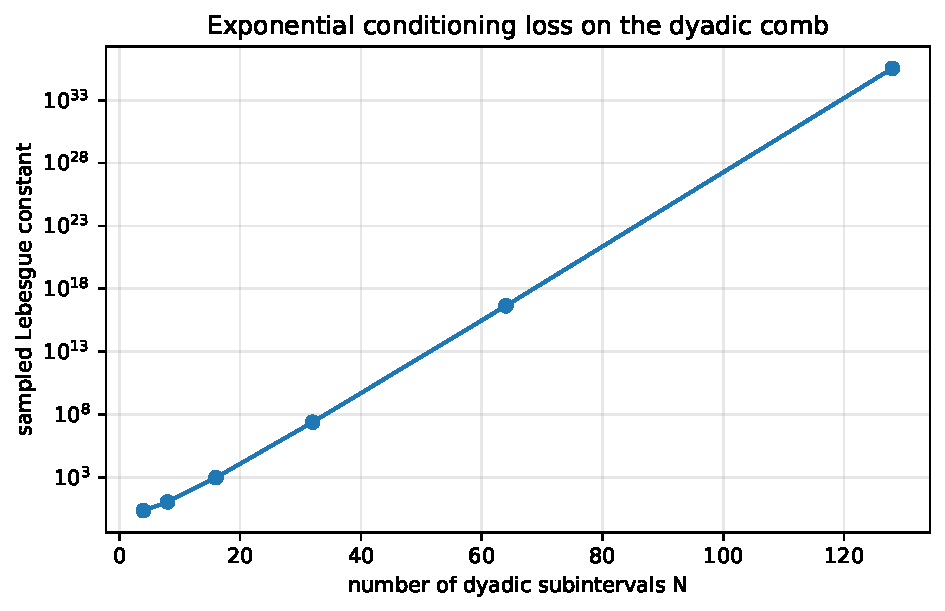
\includegraphics[width=0.82\textwidth]{figures/standard_lebesgue_growth.pdf}
\caption{Sampled Lebesgue constants.  Barycentric evaluation controls rounding in the formula, but cannot change this operator norm.}
\label{fig:standard-lebesgue}
\end{figure}
\FloatBarrier

\begin{experiment}[Observed Fabius Runge phenomenon]
\label{obs:ordinary-runge}
The sequence $P_{2^m}$ exhibits the classical endpoint oscillation of Runge's phenomenon, with errors approximately $5$, $3.6\times10^7$, and $3.8\times10^{22}$ for $N=32,64,128$.
\end{experiment}

\begin{conjecture}[Divergence of ordinary dyadic interpolation]
\label{conj:ordinary-divergence}
The global dyadic-comb interpolants satisfy
\begin{equation}
 \norm{F-P_{2^m}}_\infty\longrightarrow\infty.
 \label{eq:ordinary-divergence}
\end{equation}
A stronger plausible form is
\begin{equation}
 \frac{1}{N}\log_2\norm{F-P_N}_\infty\longrightarrow1
 \qquad(N=2^m\to\infty),
 \label{eq:ordinary-rate-conj}
\end{equation}
possibly with a subexponential, dyadically oscillatory correction.
\end{conjecture}

The operator theory makes divergence plausible but does not prove \eqref{eq:ordinary-divergence} for this specific data vector.  A proof must control cancellations between large cardinal terms weighted by the special values $F(j/N)$.

\section{Endpoint-jet deflation: an exact Hermite family}
\label{sec:jet-family}

The most natural use of the Fabius endpoint flatness is to impose derivative conditions.  The key is to do so without adding arbitrary external constraints.

\subsection{The beta-polynomial baseline}

For $r\in\N_0$, define
\begin{equation}
 S_r(x)=I_x(r+1,r+1)
 =\frac{(2r+1)!}{(r!)^2}\int_0^x t^r(1-t)^r\dd t.
 \label{eq:smoothstep}
\end{equation}
It is a polynomial of degree $2r+1$, with
\begin{align}
 S_r(0)&=0,&S_r(1)&=1,\\
 S_r^{(q)}(0)&=S_r^{(q)}(1)=0&& (1\le q\le r),\label{eq:smoothstep-jets}\\
 S_r(1-x)&=1-S_r(x).\label{eq:smoothstep-sym}
\end{align}
The first examples are $S_0=x$, $S_1=3x^2-2x^3$, and $S_2=10x^3-15x^4+6x^5$.

Set
\begin{equation}
 W_r(x)=[x(1-x)]^{r+1},
 \qquad
 g_r(x)=\frac{F(x)-S_r(x)}{W_r(x)}\quad(0<x<1).
 \label{eq:def-g}
\end{equation}
Because $F-S_r$ has zeros of order at least $r+1$ at both endpoints, $g_r$ extends to a $C^\infty$ function on $[0,1]$.  Moreover,
\begin{equation}
 g_r(1-x)=-g_r(x).
 \label{eq:g-antisym}
\end{equation}

Let $\Lag_{N-2}^{\circ}$ denote interpolation of degree at most $N-2$ on the interior nodes $j/N$, $1\le j\le N-1$.

\begin{theorem}[Endpoint-jet factorization]
\label{thm:jet-factorization}
For $N=2^m\ge4$ and $r\ge0$, define
\begin{equation}
 H_{N,r}(x)=S_r(x)+W_r(x)\,\Lag_{N-2}^{\circ}g_r(x).
 \label{eq:H-def}
\end{equation}
Then $H_{N,r}$ is the unique polynomial of degree at most $N+2r$ satisfying
\begin{align}
 H_{N,r}(j/N)&=F(j/N),&&0\le j\le N,\label{eq:H-values}\\
 H_{N,r}^{(q)}(0)&=H_{N,r}^{(q)}(1)=0,&&1\le q\le r.\label{eq:H-jets}
\end{align}
It also satisfies
\begin{align}
 H_{N,r}(1-x)&=1-H_{N,r}(x),\label{eq:H-symmetry}\\
 F(x)-H_{N,r}(x)&=W_r(x)\left(g_r(x)-\Lag_{N-2}^{\circ}g_r(x)\right).
 \label{eq:H-error-factor}
\end{align}
All coefficients are rational.  For $r=0$, $H_{N,0}=P_N$.
\end{theorem}

\begin{proof}
The interior interpolant has degree at most $N-2$, so the second term in \eqref{eq:H-def} has degree at most $N+2r$.  At an interior node, the definition of $g_r$ gives \eqref{eq:H-values}.  At $0$ and $1$, $W_r$ vanishes and $S_r$ supplies the correct endpoint values.  Since $W_r$ has zeros of order $r+1$, derivatives through order $r$ are those of $S_r$, proving \eqref{eq:H-jets}.

There are $N+1+2r=N+2r+1$ scalar conditions, exactly the dimension of polynomials of degree at most $N+2r$.  Their homogeneous version has a polynomial divisible by
\[
 x^{r+1}(1-x)^{r+1}\prod_{j=1}^{N-1}(x-j/N),
\]
of degree $N+2r+1$; hence the only homogeneous solution in degree at most $N+2r$ is zero.  This proves uniqueness.

The node set is symmetric, and \eqref{eq:g-antisym} implies that its interpolant is antisymmetric about $1/2$.  Equations \eqref{eq:smoothstep-sym} and the symmetry of $W_r$ give \eqref{eq:H-symmetry}.  Subtracting \eqref{eq:H-def} from $F=S_r+W_rg_r$ gives \eqref{eq:H-error-factor}.  Rationality follows from rational nodes, exact rational Fabius data, and rational coefficients of $S_r$.  Finally $S_0=x$ and $W_0=x(1-x)$; $H_{N,0}$ has degree at most $N$ and matches all Lagrange data, so uniqueness gives $H_{N,0}=P_N$.
\end{proof}

This theorem turns a derivative-constrained interpolation problem into ordinary interpolation of a deflated quotient.  It is not merely an approximation recipe: it is an exact characterization of the unique Hermite polynomial.

\subsection{Barycentric formula on the interior comb}

For $x_j=j/N$, $1\le j\le N-1$, take
\begin{equation}
 \omega_j=(-1)^{j-1}\binom{N-2}{j-1}.
 \label{eq:interior-weights}
\end{equation}
Then
\begin{equation}
 \Lag_{N-2}^{\circ}g_r(x)=
 \frac{\displaystyle\sum_{j=1}^{N-1}\frac{\omega_j g_r(x_j)}{x-x_j}}
 {\displaystyle\sum_{j=1}^{N-1}\frac{\omega_j}{x-x_j}}.
 \label{eq:bary-interior}
\end{equation}
Equations \eqref{eq:H-def} and \eqref{eq:bary-interior} are the computational form used in the experiments.

\section{Weighted Lebesgue geometry and an impossibility theorem}
\label{sec:weighted-lebesgue}

\subsection{The correct operator norm}

Suppose the endpoint jets remain exact, while the interior Fabius values are perturbed by $\delta_j$.  Let $\ell_j^{\circ}$ be the interior cardinal polynomials.  The resulting perturbation is
\begin{equation}
 \delta H(x)=W_r(x)\sum_{j=1}^{N-1}
 \ell_j^{\circ}(x)\frac{\delta_j}{W_r(x_j)}.
 \label{eq:perturbation}
\end{equation}
Therefore the pointwise operator norm from $\ell^\infty$ data is
\begin{equation}
 \mathscr L_{N,r}(x)=W_r(x)\sum_{j=1}^{N-1}
 \frac{\abs{\ell_j^{\circ}(x)}}{W_r(x_j)},
 \qquad
 \mathscr L_{N,r}=\norm{\mathscr L_{N,r}(\cdot)}_\infty.
 \label{eq:weighted-lebesgue}
\end{equation}
This is a weighted Lebesgue function.  The factor $W_r(x)$ suppresses perturbations near the endpoints, but division by the much smaller $W_r(x_j)$ can amplify data from nodes close to an endpoint.  The competition between these effects is the central stability issue.

\subsection{A fixed-order lower bound}

\begin{theorem}[Fixed endpoint order remains exponentially unstable]
\label{thm:fixed-r-lower}
Let $N=2^m\ge4$ and $r\ge0$.  Then
\begin{align}
 \mathscr L_{N,r}
 &\ge
 \left[\frac{2}{N}\left(1-\frac{1}{2N}\right)\right]^{r+1}
 \frac{\Gamma(N-\tfrac12)}{\sqrt\pi\,(N-2)!}
 \frac{\binom{N-2}{N/2-1}}{N/2-1/2}\label{eq:exact-lower}\\
 &=(1+o(1))\frac{2^{N+r+1/2}}{\pi N^{r+2}}
 \qquad(N\to\infty;\ r\text{ fixed}).\label{eq:fixed-asymptotic}
\end{align}
In particular, every fixed endpoint-jet order has exponential operator growth.
\end{theorem}

\begin{proof}
Evaluate one term of \eqref{eq:weighted-lebesgue} at $x=1/(2N)$ and choose the central interior node $j=N/2$.  In the scaled variable $t=Nx=1/2$,
\begin{equation}
 \abs{\ell_j^{\circ}(x)}=
 \frac{\prod_{k=1}^{N-1}\abs{t-k}}
 {\abs{t-j}(j-1)!(N-1-j)!}.
 \label{eq:cardinal-product}
\end{equation}
The numerator equals $\Gamma(N-1/2)/\sqrt\pi$.  Substituting $j=N/2$ and rewriting the factorials gives the gamma/binomial factor in \eqref{eq:exact-lower}.  The weight ratio is
\begin{equation}
 \frac{W_r(1/(2N))}{W_r(1/2)}
 =\left[\frac{2}{N}\left(1-\frac{1}{2N}\right)\right]^{r+1}.
\end{equation}
Stirling's formula and the central-binomial asymptotic yield \eqref{eq:fixed-asymptotic}.
\end{proof}

The theorem gives a necessary scale for postponement: to neutralize the factor $2^N$ in this particular lower bound, $r$ must grow at least on the order of $N/\log_2N$.  It is tempting to hope that such a growing endpoint order restores stability.  The next theorem rules that out.

\subsection{No endpoint-order schedule can stabilize the family}

Let
\begin{equation}
 \mathsf H(a)=-a\log a-(1-a)\log(1-a)
 \label{eq:entropy}
\end{equation}
be the binary entropy in natural units.

\begin{lemma}[Central cardinal growth at a fixed interior point]
\label{lem:central-cardinal}
For fixed $a\in(0,1/2)$ and even $N$,
\begin{equation}
 \frac1N\log\abs{\ell_{N/2}^{\circ}(a)}
 \longrightarrow \log2-\mathsf H(a)>0.
 \label{eq:central-cardinal-rate}
\end{equation}
\end{lemma}

\begin{proof}
Write the cardinal product in gamma functions, or apply Stirling's formula separately to the products to the left and right of $aN$.  The denominator has the central entropy rate $\mathsf H(1/2)=\log2$, while the numerator removes the rate $\mathsf H(a)$, giving \eqref{eq:central-cardinal-rate}.
\end{proof}

\begin{theorem}[All-order exponential barrier]
\label{thm:all-r-barrier}
There exist absolute constants $c>0$ and $N_0$ such that, for every dyadic $N\ge N_0$ and every integer $r\ge0$,
\begin{equation}
 \mathscr L_{N,r}\ge \exp(cN).
 \label{eq:all-r-barrier}
\end{equation}
Consequently, no choice $r=r_N$ of endpoint derivative order makes the family $H_{N,r_N}$ uniformly stable as an interpolation operator on the dyadic comb.
\end{theorem}

\begin{proof}
Fix a small $\varepsilon>0$ and split into two regimes.

\emph{Moderate jet order.}  Suppose
\begin{equation}
 r\le \frac{(\log2+\varepsilon)N}{\log N}.
 \label{eq:moderate-r}
\end{equation}
Evaluate \eqref{eq:weighted-lebesgue} at a fixed point, say $a=1/10$, and retain the central term $j=N/2$.  The weight ratio is
\begin{equation}
 \frac{W_r(a)}{W_r(1/2)}=[4a(1-a)]^{r+1}.
\end{equation}
Its logarithm is $\bigO(r)=o(N)$ under \eqref{eq:moderate-r}.  By \Cref{lem:central-cardinal}, the cardinal factor contributes
\[
 \exp\bigl(N(\log2-\mathsf H(1/10)+o(1))\bigr),
\]
with strictly positive exponential rate.  Thus \eqref{eq:all-r-barrier} holds in this regime.

\emph{Large jet order.}  Put
\begin{equation}
 x=\frac{N+1}{2N},\qquad j=1.
\end{equation}
A direct gamma-product calculation gives the exact cardinal value
\begin{equation}
 \abs{\ell_1^{\circ}\!\left(\frac{N+1}{2N}\right)}
 =\frac{\binom{N-2}{N/2-1}}{16^{N/2-1}}
 =(1+o(1))\frac{2^{-N+2}}{\sqrt{\pi N/2}}.
 \label{eq:endpoint-cardinal}
\end{equation}
The weight ratio is especially simple:
\begin{equation}
 \frac{x(1-x)}{(1/N)(1-1/N)}=\frac{N+1}{4}.
 \label{eq:large-r-ratio}
\end{equation}
Hence one term of $\mathscr L_{N,r}$ is bounded below by
\begin{equation}
 \left(\frac{N+1}{4}\right)^{r+1}
 \frac{\binom{N-2}{N/2-1}}{16^{N/2-1}}.
 \label{eq:large-r-lower}
\end{equation}
If \eqref{eq:moderate-r} fails, then for sufficiently large $N$ the logarithm of \eqref{eq:large-r-lower} is at least $\varepsilon N/3$.  Indeed, $\log((N+1)/4)=(1+o(1))\log N$, while the cardinal term contributes $-N\log2+o(N)$.  Combining the two regimes and reducing $c$ if necessary proves the theorem.
\end{proof}

\begin{remark}[What the theorem does and does not prove]
\Cref{thm:all-r-barrier} is an operator result.  It proves that endpoint derivative constraints cannot create a uniformly stable interpolation process on arbitrary nearby data.  It does not by itself prove that the exact Fabius data excite the worst direction for every $N$.  The numerical results in the next section show that they eventually do excite very large oscillations.
\end{remark}

\section{How much do endpoint jets help in practice?}
\label{sec:jet-numerics}

\subsection{Error scans}

At moderate $N$, increasing $r$ initially produces a dramatic improvement.  At $N=32$, the error falls from approximately $4.99$ to $7.62\times10^{-7}$ at $r=8$, an improvement by more than six million.  It then rises again.

\begin{table}[htbp]
\centering
\caption{Selected endpoint-jet errors and weighted Lebesgue constants.}
\label{tab:jet-selected}
\small
\begin{tabular}{rrrrr}
\toprule
$N$ & $r$ & degree $N+2r$ & $\norm{F-H_{N,r}}_\infty$ & $\mathscr L_{N,r}$ \\
\midrule
32 & 0  & 32  & $4.989$ & $2.431\times10^7$ \\
32 & 4  & 40  & $1.111\times10^{-4}$ & $8.908\times10^2$ \\
32 & 8  & 48  & $7.623\times10^{-7}$ & $1.298\times10^1$ \\
32 & 10 & 52  & $6.055\times10^{-6}$ & $4.373\times10^1$ \\
\addlinespace
64 & 8  & 80  & $4.764\times10^{-3}$ & $6.403\times10^6$ \\
64 & 12 & 88  & $8.303\times10^{-6}$ & $1.292\times10^4$ \\
64 & 14 & 92  & $1.777\times10^{-6}$ & $2.825\times10^3$ \\
64 & 17 & 98  & $4.907\times10^{-4}$ & $2.580\times10^5$ \\
\addlinespace
128 & 20 & 168 & $1.570\times10^{-1}$ & $5.057\times10^{11}$ \\
128 & 23 & 174 & $3.978\times10^{-3}$ & $6.189\times10^9$ \\
128 & 26 & 180 & $1.087$ & $3.356\times10^{11}$ \\
\addlinespace
256 & 39 & 334 & $3.295\times10^9$ & $2.145\times10^{25}$ \\
256 & 40 & 336 & $9.327\times10^8$ & $4.279\times10^{24}$ \\
256 & 41 & 338 & $4.511\times10^9$ & $2.747\times10^{24}$ \\
256 & 42 & 340 & $5.652\times10^{10}$ & $2.478\times10^{25}$ \\
\bottomrule
\end{tabular}
\end{table}

\begin{figure}[htbp]
\centering
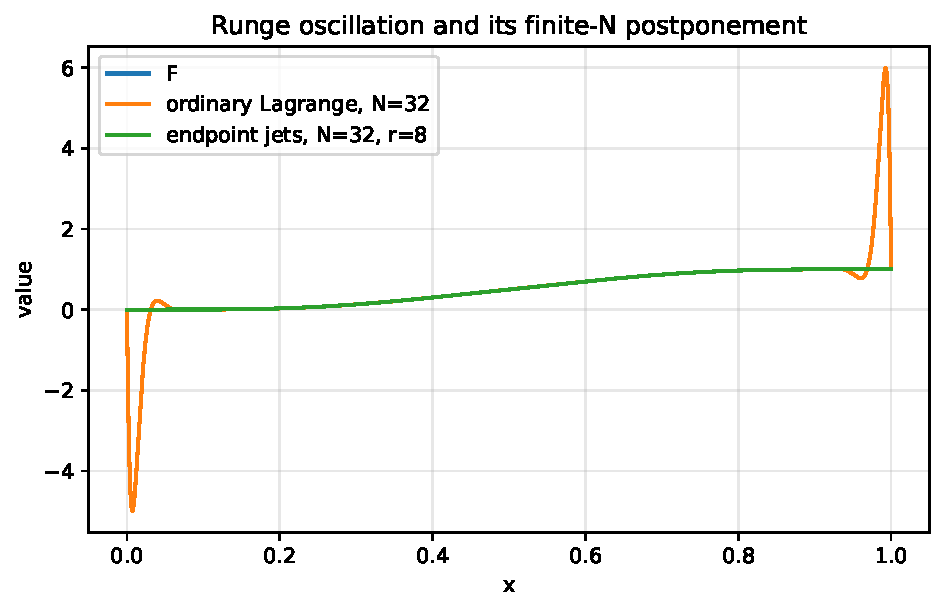
\includegraphics[width=0.82\textwidth]{figures/interpolants_N32.pdf}
\caption{At $N=32$, endpoint jets suppress the visible global oscillation at finite $N$.  This is postponement, not asymptotic stabilization.}
\label{fig:interpolants32}
\end{figure}

\begin{figure}[htbp]
\centering
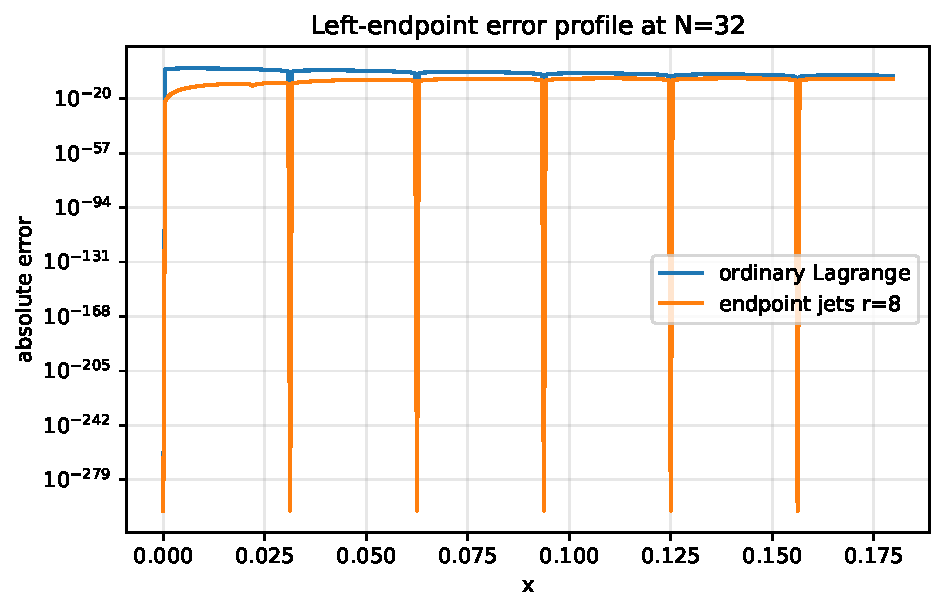
\includegraphics[width=0.82\textwidth]{figures/endpoint_error_profile_N32.pdf}
\caption{The ordinary error is concentrated near the endpoint.  Jet deflation moves and reduces the dominant peak.}
\label{fig:endpoint-profile}
\end{figure}
\FloatBarrier

The scans are U-shaped in $r$: too few jets leave the usual endpoint instability, while too many jets amplify the factors $W_r(x)/W_r(x_j)$ associated with near-endpoint nodes.

\begin{figure}[htbp]
\centering
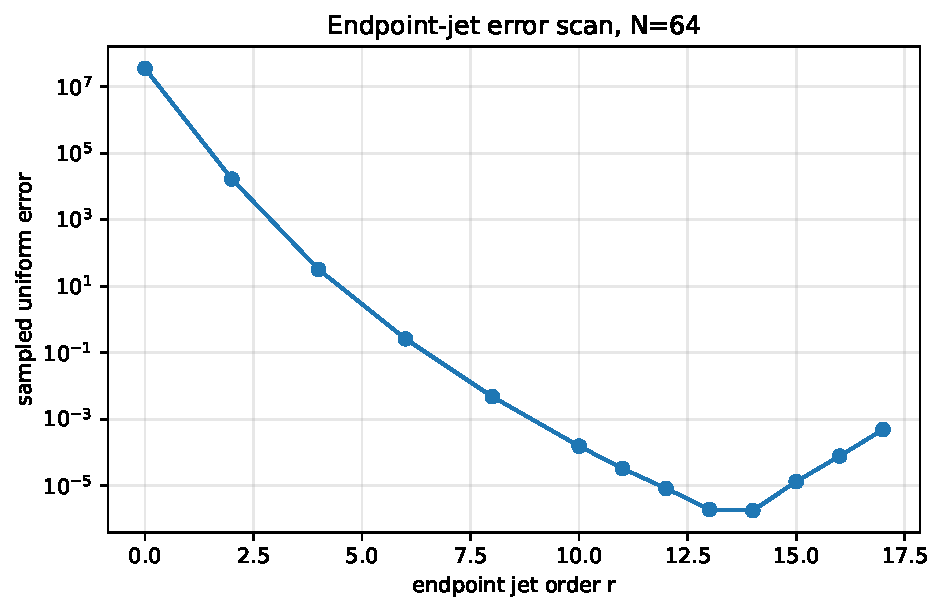
\includegraphics[width=0.78\textwidth]{figures/jet_error_scan_N64.pdf}
\caption{Error as a function of endpoint order for $N=64$.}
\label{fig:scan64}
\end{figure}

\begin{figure}[htbp]
\centering
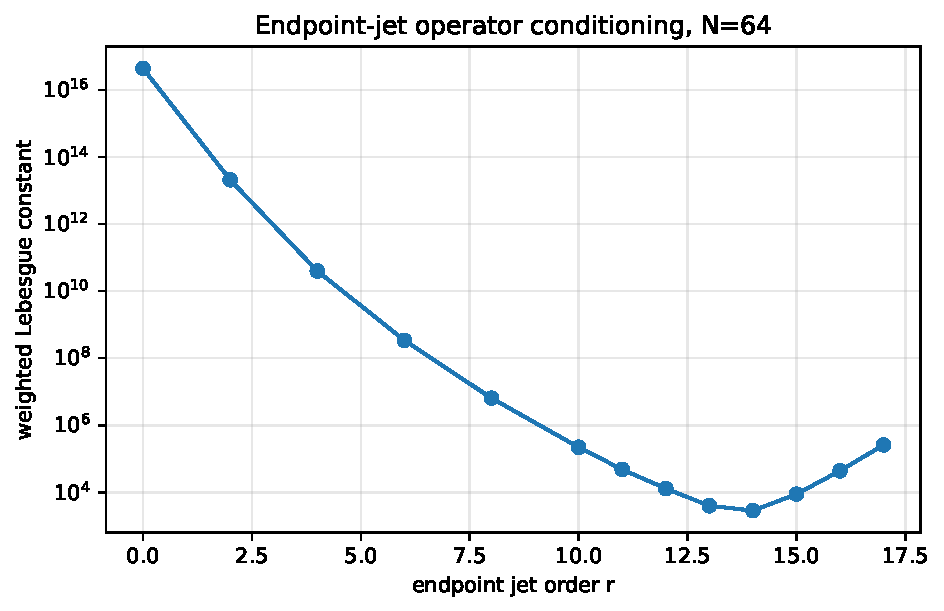
\includegraphics[width=0.78\textwidth]{figures/jet_weighted_lebesgue_N64.pdf}
\caption{The weighted Lebesgue constant has its minimum near the same order as the actual Fabius error at $N=64$.}
\label{fig:lebesgue64}
\end{figure}
\FloatBarrier

\subsection{A two-mechanism balance law}

The two terms used in the proofs of \Cref{thm:fixed-r-lower,thm:all-r-barrier} also predict the finite-$N$ optimum.  On a base-$2$ logarithmic scale, the central-node/near-endpoint mechanism behaves roughly as
\begin{equation}
 A_{N,r}:\quad N-r(\log_2N-1),
 \label{eq:mechanism-A}
\end{equation}
whereas the endpoint-node/near-center mechanism behaves roughly as
\begin{equation}
 B_{N,r}:\quad -N+r(\log_2N-2).
 \label{eq:mechanism-B}
\end{equation}
Balancing \eqref{eq:mechanism-A} and \eqref{eq:mechanism-B} gives
\begin{equation}
 r_{\mathrm{bal}}(N)=\frac{2N}{2\log_2N-3}
 =\frac{N}{\log_2N-3/2}.
 \label{eq:r-balance}
\end{equation}

\begin{table}[htbp]
\centering
\caption{Observed optimal endpoint orders versus the balance law.  The scans are discrete and finite, so agreement to one or two units is the appropriate standard.}
\label{tab:optimal-r}
\begin{tabular}{rrrrr}
\toprule
$N$ & error-optimal $r$ & minimum sampled error & stability-optimal $r$ & $r_{\mathrm{bal}}(N)$ \\
\midrule
16  & 5  & $2.734\times10^{-5}$ & 5  & 6.40 \\
32  & 8  & $7.623\times10^{-7}$ & 8  & 9.14 \\
64  & 14 & $1.777\times10^{-6}$ & 14 & 14.22 \\
128 & 23 & $3.978\times10^{-3}$ & 23 & 23.27 \\
256 & 40 & $9.327\times10^{8}$ & 41 & 39.38 \\
\bottomrule
\end{tabular}
\end{table}

\begin{conjecture}[Asymptotically optimal endpoint order]
\label{conj:optimal-r}
Let $r_N^{\mathrm{op}}$ minimize $\mathscr L_{N,r}$ over integers $r\ge0$.  Then
\begin{equation}
 r_N^{\mathrm{op}}=\frac{N}{\log_2N-3/2}
 +o\!\left(\frac{N}{(\log N)^2}\right).
 \label{eq:optimal-r-conj}
\end{equation}
At the weaker level,
\begin{equation}
 \frac{r_N^{\mathrm{op}}\log_2N}{N}\longrightarrow1.
 \label{eq:optimal-r-weak}
\end{equation}
The same leading law is expected for the order minimizing the actual Fabius error, though lower-order dyadic oscillations may shift it by several integers.
\end{conjecture}

\begin{conjecture}[Optimized endpoint jets still diverge]
\label{conj:optimized-divergence}
If
\begin{equation}
 E_N^*=\min_{r\ge0}\norm{F-H_{N,r}}_\infty,
\end{equation}
then $E_{2^m}^*\to\infty$.  More strongly, $\log E_N^*$ is expected to be linear in $N$ up to $o(N)$ terms.
\end{conjecture}

The data at $N=256$ provide the first unambiguous sign of this second divergence regime: optimization over endpoint flatness no longer produces a useful approximation.

\section{Matching derivatives at every dyadic node}
\label{sec:full-hermite}

The phrase ``fixing higher derivatives'' may also mean imposing derivative data at every comb point, not merely at the two endpoints.  This produces a confluent Hermite polynomial.

For $q\ge0$, let $K_{N,q}$ be the unique polynomial of degree at most
\begin{equation}
 d_{N,q}=(q+1)(N+1)-1
 \label{eq:full-hermite-degree}
\end{equation}
that satisfies
\begin{equation}
 K_{N,q}^{(s)}(j/N)=F^{(s)}(j/N),
 \qquad 0\le j\le N,\quad0\le s\le q.
 \label{eq:full-hermite-conditions}
\end{equation}
The derivative tower \eqref{eq:derivative-tower} implies that every datum is rational:
\begin{equation}
 F^{(s)}(j/N)=2^{\binom{s+1}{2}}\Fext(2^s j/N)\in\Q.
 \label{eq:dyadic-derivatives}
\end{equation}
Thus the full-grid Hermite polynomial is also exactly defined over $\Q$.

The numerical result is negative.

\begin{table}[htbp]
\centering
\caption{Full-grid Hermite interpolation.  Here $q$ means that derivatives $0,1,\ldots,q$ are matched at every node.}
\label{tab:full-hermite}
\begin{tabular}{rrrrr}
\toprule
$N$ & $q$ & degree & sampled max error & left maximizer \\
\midrule
4  & 1 & 9  & $1.148\times10^{-2}$ & 0.093994 \\
4  & 2 & 14 & $6.555\times10^{-3}$ & 0.099365 \\
4  & 3 & 19 & $6.887\times10^{-3}$ & 0.092285 \\
8  & 1 & 17 & $3.736\times10^{-3}$ & 0.040283 \\
8  & 2 & 26 & $4.435\times10^{-3}$ & 0.040771 \\
8  & 3 & 35 & $2.735\times10^{-1}$ & 0.037842 \\
16 & 1 & 33 & $2.272$ & 0.016113 \\
16 & 2 & 50 & $5.089\times10^{2}$ & 0.016357 \\
32 & 1 & 65 & $1.538\times10^{7}$ & 0.007080 \\
\bottomrule
\end{tabular}
\end{table}

\begin{figure}[htbp]
\centering
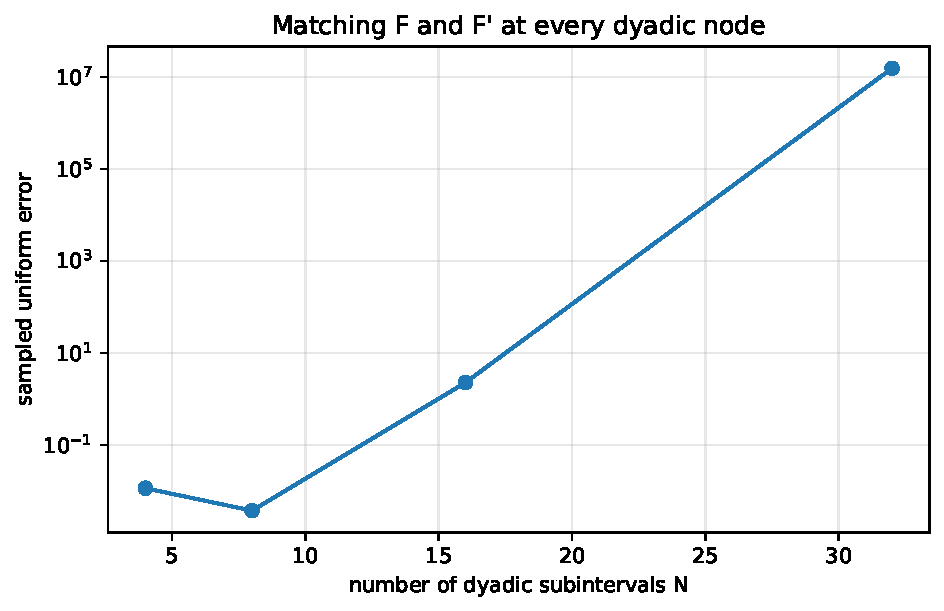
\includegraphics[width=0.80\textwidth]{figures/full_grid_hermite_error.pdf}
\caption{Matching only the first derivative at every dyadic node causes an earlier Runge explosion because the polynomial degree nearly doubles while the nodes remain equispaced.}
\label{fig:full-hermite}
\end{figure}
\FloatBarrier

These computations align with classical results that Hermite and Fejer operators on equispaced nodes can also have exponentially growing norms \cite{manni}.  Derivative information is valuable only when paired with an approximation architecture that controls global degree and node geometry; simply adding confluent conditions to every equispaced node is not a cure.

\section{The Rvachev function on half and full combs}
\label{sec:rvachev}

\subsection{Half-support interpolation is a translation}

On $[-1,0]$, $\Up(y)=F(y+1)$.  Therefore the interpolation problem on
\begin{equation}
 y_j=-1+j/N,
 \qquad0\le j\le N,
\end{equation}
is exactly the Fabius problem under $x=y+1$.  Every result above, including the jet factorization and weighted lower bounds, transfers without change.

\subsection{Full symmetric comb and even reduction}

Consider the full comb
\begin{equation}
 y_j=\frac{j}{N},\qquad -N\le j\le N,
\end{equation}
and let $R_N$ be the unique degree-$2N$ interpolant to $\Up(y_j)$.

\begin{proposition}[Even-polynomial reduction]
\label{prop:even-reduction}
The polynomial $R_N$ is even.  Hence there is a unique polynomial $Q_N$ of degree at most $N$ such that
\begin{equation}
 R_N(y)=Q_N(y^2),
 \end{equation}
and
\begin{equation}
 Q_N\!\left(\frac{j^2}{N^2}\right)=\Up(j/N),
 \qquad 0\le j\le N.
 \label{eq:squared-grid}
\end{equation}
\end{proposition}

\begin{proof}
The data and node set are invariant under $y\mapsto-y$.  Uniqueness forces $R_N(-y)=R_N(y)$.  Every even polynomial of degree at most $2N$ is a polynomial of degree at most $N$ in $y^2$; evaluating at $j/N$ gives \eqref{eq:squared-grid}.
\end{proof}

Thus the symmetric full-comb problem is equivalent to interpolation on the quadratically spaced nodes $j^2/N^2$ in the variable $z=y^2$.  This exact reduction is useful for both analysis and computation.

\subsection{Endpoint jets for $\Up$}

Since $\Up$ and all its derivatives vanish at $\pm1$, no nonzero smoothstep baseline is needed.  Define
\begin{equation}
 \Gamma_r(y)=\frac{\Up(y)}{(1-y^2)^{r+1}}.
 \label{eq:gamma-up}
\end{equation}
It extends smoothly to $[-1,1]$ and is even.  Let $\Lag^{\circ}_{2N-2}$ interpolate on the $2N-1$ interior nodes $j/N$, $|j|<N$.

\begin{theorem}[Rvachev endpoint-jet interpolant]
\label{thm:up-jet}
The polynomial
\begin{equation}
 U_{N,r}(y)=(1-y^2)^{r+1}\Lag^{\circ}_{2N-2}\Gamma_r(y)
 \label{eq:up-jet}
\end{equation}
has degree at most $2N+2r$, matches $\Up$ at all $2N+1$ nodes, and matches derivatives through order $r$ at both endpoints.  It is the unique polynomial with these properties and is even.  Equivalently,
\begin{equation}
 U_{N,r}(y)=(1-y^2)^{r+1}\widetilde Q_{N,r}(y^2)
\end{equation}
for a polynomial $\widetilde Q_{N,r}$ of degree at most $N-1$.
\end{theorem}

The weighted Lebesgue analysis is affinely invariant, so the exponential instability mechanisms of \Cref{thm:fixed-r-lower,thm:all-r-barrier} persist on the full Rvachev comb.  Evenness halves the algebraic dimension but does not change the underlying equispaced geometry in $y$.

\section{Asymptotic peak migration and Lambert $W$}
\label{sec:lambert}

The repository develops detailed endpoint asymptotics involving lower branches of Lambert $W$.  A related Lambert structure appears in the interpolation instability itself.

For a central cardinal term evaluated at $x\in(0,1/2)$ and jet ratio $\rho=r/N$, a formal exponential rate has the shape
\begin{equation}
 \Phi_\rho(x)=\log2-\mathsf H(x)+\rho\log(4x(1-x)).
 \label{eq:rate-function}
\end{equation}
A saddle satisfies
\begin{equation}
 \Phi_\rho'(x)=
 \log\frac{x}{1-x}+\rho\frac{1-2x}{x(1-x)}=0.
 \label{eq:saddle-equation}
\end{equation}
When $\rho\downarrow0$ and the saddle lies near the endpoint, the leading balance is
\begin{equation}
 x\log(1/x)\sim\rho.
\end{equation}
Hence
\begin{equation}
 x_\rho\sim -\frac{\rho}{W_{-1}(-\rho)}.
 \label{eq:lambert-peak}
\end{equation}
This gives a conceptual bridge between the endpoint Lambert asymptotics of $F$ itself and the migration of the interpolation error peak.

\begin{conjecture}[Lambert peak law]
\label{conj:lambert-peak}
In a regime $r/N\to0$ with $r\to\infty$, the dominant weighted-cardinal peak associated with central nodes is located at
\begin{equation}
 x_{N,r}= -\frac{r/N}{W_{-1}(-r/N)}\left(1+o(1)\right),
 \end{equation}
up to a bounded log-periodic modulation induced by the dyadic structure of the exact Fabius data.
\end{conjecture}

A full saddle expansion of \eqref{eq:rate-function} would naturally involve Bernoulli polynomials through Stirling/Euler--Maclaurin corrections and Bell polynomials through composition with the Lambert expansion.  This offers a concrete route for connecting the interpolation problem to several themes already developed in the repository without repeating their existing formulas.

\section{Why local dyadic reconstruction behaves differently}
\label{sec:local-global}

The negative results concern a \emph{single global polynomial} whose degree grows proportionally to the number of equispaced samples.  They do not contradict the stable dyadic schemes already present in the repository.

A piecewise-linear interpolant uses only two neighboring samples in each cell.  Its Lebesgue constant is $1$, its error is controlled locally by $F''$, and the representation/Faber--Schauder material in the corpus obtains algebraic $4^{-m}$-scale errors.  Repeated integration produces higher-order local splines with similarly controlled support.  In contrast, the global cardinal polynomial attached to one node is nonzero across the entire interval, and the equispaced Lebesgue constant is exponential.

This distinction suggests a practical hierarchy:
\begin{enumerate}[leftmargin=2em]
\item exact dyadic evaluation for data generation;
\item local piecewise polynomial or compactly supported atomic reconstruction for stability;
\item global polynomial approximation only with degree substantially below the sample count, or with a change of basis/node geometry;
\item global interpolation at all dyadic nodes only for small $N$ or exact symbolic identities, not as an asymptotic approximation scheme.
\end{enumerate}

\section{Alternative stable or nearly stable directions}
\label{sec:alternatives}

\subsection{Oversampled least squares}

Use $M+1$ dyadic samples but fit a polynomial of degree $n\ll M$.  The Coppersmith--Rivlin and Platte--Trefethen--Kuijlaars theory indicates that stable high-order approximation from equispaced samples requires oversampling; root-exponential regimes and positive results are discussed in \cite{platte-trefethen-kuijlaars,adcock-shadrin}.  The exact Fabius samples make this especially attractive because data noise can be separated from conditioning exactly.

\subsection{Mock-Chebyshev extraction}

Select from the fine dyadic comb a subset nearest to Chebyshev nodes, then interpolate or constrain a least-squares fit.  Recent constrained mock-Chebyshev methods extend this idea to Hermite data \cite{mock-chebyshev-hermite}.  The dyadic derivative tower supplies exact derivative samples, but the polynomial degree must remain tied to the selected near-Chebyshev subset rather than the full comb.

\subsection{Barycentric rational Hermite interpolation}

Floater--Hormann-type rational interpolants can have logarithmic rather than exponential Lebesgue growth on equidistant nodes, and rational Hermite variants retain derivative data \cite{cirillo-hormann}.  The absence of real poles in appropriate parameter ranges makes this a promising direct successor to the failed polynomial Hermite experiments.

\subsection{Shape and endpoint constrained minimax approximation}

Instead of interpolation, solve a constrained minimax or least-squares problem with
\begin{equation}
 p(0)=0,\quad p(1)=1,\quad p^{(q)}(0)=p^{(q)}(1)=0,
 \end{equation}
while allowing residuals at interior dyadic nodes.  The beta baseline $S_r$ remains useful: write $p=S_r+W_rq$ and approximate $g_r$ in a stable basis such as Chebyshev polynomials.  This preserves endpoint flatness without inheriting the interior equispaced interpolation operator.

\subsection{Atomic and Faber--Schauder bases}

The Rvachev function was historically developed precisely as a compactly supported atomic basis for approximation.  A basis adapted to the refinement equation and dyadic support is more natural than a monomial basis for this function.  The repository's exact tent coefficients provide a starting point for adaptive truncation and certified local error control.

\section{Further conjectures and research directions}
\label{sec:future}

\begin{conjecture}[Dyadic modulation of global interpolation error]
After subtracting a smooth leading exponential rate from $\log\norm{F-P_{2^m}}_\infty$, the residual has a nonconstant bounded oscillation in a lower-Lambert or binary phase, analogous to the endpoint periodic correction already proved for $F$ itself.
\end{conjecture}

\begin{conjecture}[$2$-adic stability counterpart]
Although the real Lebesgue constants are exponential, the exact valuation law \eqref{eq:weight-valuation} permits a renormalized $2$-adic interpolation operator on dyadic data with substantially better norm growth.  A natural problem is to identify the correct Mahler-type basis and compare it with the ordinary binomial Newton form \eqref{eq:newton-forward}.
\end{conjecture}

\begin{question}[Exact sign/cancellation structure]
Can the signs or valuations of the forward differences
\begin{equation}
 \Delta^kF(0)=\sum_{j=0}^{k}(-1)^{k-j}\binom kjF(j/N)
\end{equation}
be described by a Thue--Morse or $q$-binomial law when $N=2^m$?  Such a law could turn the numerical divergence conjecture into a rigorous lower bound by controlling cancellations in \eqref{eq:newton-forward}.
\end{question}

\begin{question}[Inverse Fabius interpolation]
The inverse function has infinite endpoint slopes rather than flatness.  What is the exact analogue of jet deflation after the nonlinear change of variables suggested by the inverse Lambert asymptotics?  Direct equispaced interpolation in the probability variable is expected to be even more delicate.
\end{question}

\begin{question}[Formal verification]
The following results are realistic Lean targets: the endpoint-jet factorization, rationality and symmetry, the exact cardinal values in \eqref{eq:exact-lower} and \eqref{eq:endpoint-cardinal}, and the all-order exponential barrier.  The proofs use only polynomial uniqueness, finite products, gamma/binomial identities, and elementary asymptotics, all close to infrastructure already present in the repository.
\end{question}

Other promising tasks include:
\begin{itemize}[leftmargin=2em]
\item a complete saddle-point expansion of $\mathscr L_{N,r}$ with Bernoulli corrections;
\item certified interval-arithmetic maxima, replacing sampled maxima in the numerical tables;
\item optimal oversampling laws for Fabius-specific least squares, exploiting exact dyadic values;
\item comparison of polynomial, rational, spline, atomic, and Faber--Schauder reconstructions at equal arithmetic cost;
\item a spectral analysis of the interpolation error using the infinite sinc product for $\widehat{\Up}$;
\item a $q$-deformation interpolating between the additive dyadic comb and the geometric nodes already used in the repository's $q$-series coefficient extractors.
\end{itemize}

\section{Computational methodology and reproducibility}
\label{sec:computation}

The accompanying file
\begin{center}
\path{fabius_dyadic_interpolation_experiments.py}
\end{center}
contains detailed comments and regenerates the CSV tables and figures.  Its main safeguards are:
\begin{enumerate}[leftmargin=2em]
\item \textbf{Exact inputs.}  Values $F(a/2^e)$ and all derivative data are computed as rational numbers using \eqref{eq:V-recurrence}--\eqref{eq:bit-split} and the derivative recursion from \eqref{eq:F-dde}.
\item \textbf{High precision.}  Barycentric evaluation uses \texttt{mpmath}, with precision increasing to more than $200$ decimal digits for the largest reported cases.  Double precision would confound mathematical Runge growth with rounding error.
\item \textbf{Symmetry.}  Only $[0,1/2]$ is searched; the other half follows exactly from \eqref{eq:P-symmetry} and \eqref{eq:H-symmetry}.
\item \textbf{Independent formulations.}  Ordinary Lagrange interpolation is checked both directly and as $H_{N,0}$.  Full-grid Hermite interpolation uses confluent Newton divided differences with exact repeated-node derivatives.
\item \textbf{Grid disclosure.}  Ordinary errors use spacing $2^{-13}$; endpoint-jet scans use $2^{-12}$ through $N=128$ and $2^{-11}$ at $N=256$; full-grid Hermite uses $2^{-12}$.  The maxima are therefore sampled lower bounds on the true uniform errors, not interval-certified maxima.
\end{enumerate}

The code also writes the raw data files
\begin{itemize}[leftmargin=2em]
\item \path{results/standard_lagrange.csv},
\item \path{results/endpoint_jet_scan.csv},
\item \path{results/optimal_jet_orders.csv},
\item \path{results/full_grid_hermite.csv}.
\end{itemize}

\section{Conclusions}
\label{sec:conclusions}

The Fabius function combines exact dyadic arithmetic with extreme nonanalytic smoothness, making it an unusually clean laboratory for separating data accuracy from interpolation stability.  The central conclusions are:
\begin{enumerate}[leftmargin=2em]
\item Ordinary global Lagrange interpolation on the dyadic comb shows severe Runge behavior.  Exact samples do not protect against an exponentially bad interpolation operator.
\item Endpoint flatness can be imposed exactly through the beta-polynomial factorization \eqref{eq:H-def}.  This produces a transparent Hermite family in which ordinary Lagrange interpolation is the zeroth member.
\item Fixed endpoint order is exponentially unstable, and even an order growing with $N$ cannot stabilize the operator.  The all-order barrier is a rigorous negative result.
\item A balanced order near $N/(\log_2N-3/2)$ can postpone the visible catastrophe.  It is a useful finite-$N$ tuning law, not an asymptotic cure.
\item Matching derivatives at every dyadic node is counterproductive because it increases the global degree without changing the equispaced geometry.
\item The full Rvachev problem inherits the same instability, with an additional exact even-polynomial reduction.
\item Stable future methods should keep the exact dyadic data but abandon full-degree global polynomial interpolation: local atomic/spline bases, oversampled least squares, mock-Chebyshev subsets, rational Hermite formulas, or constrained minimax approximation are the natural alternatives.
\end{enumerate}

The most promising theoretical frontier is to combine the exact dyadic arithmetic with saddle analysis of the weighted cardinal functions.  That program should reveal Lambert-$W$ peak laws, Bernoulli/Bell correction hierarchies, and possibly a Thue--Morse description of the cancellations that determine the actual, rather than worst-case, interpolation error.

\appendix

\section{Proof details for the cardinal values}
\label{app:cardinal}

For interior nodes $1/N,\dots,(N-1)/N$, put $t=Nx$.  The cardinal polynomial is
\begin{equation}
 \ell_j^{\circ}(x)=
 \frac{\prod_{1\le k\le N-1,\,k\ne j}(t-k)}
 {\prod_{1\le k\le N-1,\,k\ne j}(j-k)}.
\end{equation}
Taking absolute values gives \eqref{eq:cardinal-product}.  At $t=1/2$,
\begin{equation}
 \prod_{k=1}^{N-1}\left(k-\frac12\right)
 =\frac{\Gamma(N-1/2)}{\Gamma(1/2)}.
\end{equation}
For $j=N/2$ this becomes
\begin{equation}
 \abs{\ell_{N/2}^{\circ}(1/(2N))}
 =\frac{\Gamma(N-1/2)}{\sqrt\pi(N-2)!}
 \frac{\binom{N-2}{N/2-1}}{N/2-1/2}.
\end{equation}

For the second exact value, write $N=2M$, $t=M+1/2$, and $j=1$.  The products on the two sides of the half-integer give
\begin{align}
 \abs{\ell_1^{\circ}((N+1)/(2N))}
 &=\frac{\Gamma(M+1/2)\Gamma(M-1/2)}
 {\pi(M-1/2)(2M-2)!}\\
 &=\frac{\Gamma(M-1/2)^2}{\pi(2M-2)!}\\
 &=\frac{(2M-2)!}{16^{M-1}(M-1)!^2}\\
 &=\frac{\binom{N-2}{N/2-1}}{16^{N/2-1}}.
\end{align}
These identities are exact and involve no approximation of $F$.

\section{A compact pseudocode summary}
\label{app:pseudocode}

\begin{lstlisting}[language=Python,caption={Endpoint-jet interpolation in barycentric form.}]
# N is a power of two; nodes are x_j=j/N, j=1,...,N-1.
# F(x_j) is evaluated exactly as a Fraction.

def S(r, x):
    C = factorial(2*r+1) / factorial(r)**2
    return C * sum((-1)**k * binomial(r,k)
                   * x**(r+k+1)/(r+k+1)
                   for k in range(r+1))

W = lambda r, x: (x*(1-x))**(r+1)
g_j = [(F(x_j)-S(r,x_j))/W(r,x_j) for x_j in nodes]
w_j = [(-1)**(j-1)*binomial(N-2,j-1) for j in range(1,N)]

q = barycentric(x, nodes, g_j, w_j)
H = S(r,x) + W(r,x)*q
\end{lstlisting}

\section{Repository non-duplication checklist}
\label{app:nondup}

\begin{longtable}{@{}p{0.30\textwidth}p{0.64\textwidth}@{}}
\toprule
Corpus topic & Relation to this report \\
\midrule
\endfirsthead
\toprule
Corpus topic & Relation to this report \\
\midrule
\endhead
Exact dyadic evaluator & Reused as an input oracle; no new claim of discovering the evaluator. \\
Derivative tower and endpoint flatness & Reused to define and justify the jet quotient $g_r$. \\
Thue--Morse and $q$-binomial identities & Not duplicated; this report adds ordinary-binomial barycentric weights and their exact $2$-adic valuation law. \\
Geometric-node Lagrange formulas & Distinct: those are $q$-series coefficient extractors, whereas the present nodes are additive and equispaced. \\
Piecewise-linear/Faber--Schauder reconstruction & Distinct and used as a stable local benchmark, not rederived. \\
Repeated-integration splines & Distinct local approximants; the present object is one global polynomial. \\
Lambert endpoint asymptotics & Not duplicated; the new Lambert appearance is the cardinal-saddle peak law \eqref{eq:lambert-peak}. \\
Inverse Fabius asymptotics & Used only to motivate a future interpolation problem. \\
Fourier/sinc product representations & Suggested as an independent reference and spectral-error route; no duplicate representation theorem is claimed. \\
Global Lagrange Runge study & Not found in the audited corpus; this is the principal new subject. \\
Endpoint beta-polynomial jet factorization & Not found in the audited corpus; proved in \Cref{thm:jet-factorization}. \\
All-order endpoint-jet instability & Not found in the audited corpus; proved in \Cref{thm:all-r-barrier}. \\
\bottomrule
\end{longtable}

\begin{thebibliography}{99}

\bibitem{jessen1935}
B.~Jessen and A.~Wintner,
\newblock Distribution functions and the Riemann zeta function,
\newblock \emph{Transactions of the American Mathematical Society} \textbf{38} (1935), 48--88.

\bibitem{fabius1966}
J.~Fabius,
\newblock A probabilistic example of a nowhere analytic $C^\infty$-function,
\newblock \emph{Zeitschrift fuer Wahrscheinlichkeitstheorie und Verwandte Gebiete} \textbf{5} (1966), 173--174.
\newblock DOI: \nolinkurl{10.1007/BF00536652}.

\bibitem{rvachev1971}
V.~L.~Rvachev and V.~A.~Rvachev,
\newblock A certain finite function,
\newblock \emph{Dopovidi Akademii Nauk Ukrains'koi RSR, Series A} (1971), 705--707, 764.

\bibitem{rvachev1990}
V.~A.~Rvachev,
\newblock Compactly supported solutions of functional-differential equations and their applications,
\newblock \emph{Russian Mathematical Surveys} \textbf{45} (1990), no.~1, 87--120.

\bibitem{arias1982}
J.~Arias de Reyna,
\newblock An infinitely differentiable function with compact support: definition and properties,
\newblock English translation of the 1982 Spanish paper, arXiv:\nolinkurl{1702.05442} (2017).

\bibitem{arias2018}
J.~Arias de Reyna,
\newblock Arithmetic of the Fabius function,
\newblock \emph{INTEGERS} \textbf{18} (2018), Article A51; arXiv:\nolinkurl{1702.06487}, version 3.

\bibitem{haugland2016}
J.~K.~Haugland,
\newblock Evaluating the Fabius function,
\newblock arXiv:\nolinkurl{1609.07999} (2016).

\bibitem{proveit-primary}
V.~Reshetnikov,
\newblock \emph{Fabius Function and Rvachev Up}, primary exposition in the ProveIt repository,
\newblock consulted 28 August 2026,
\newblock \url{https://github.com/VladimirReshetnikov/ProveIt/tree/main/Analysis/FabiusFunction/docs/Fabius_Function_and_Rvachev_Up}.

\bibitem{proveit-frontiers}
V.~Reshetnikov,
\newblock \emph{Non-formalized research frontiers for the Fabius--Rvachev system},
\newblock ProveIt repository, consulted 28 August 2026,
\newblock \url{https://github.com/VladimirReshetnikov/ProveIt/tree/main/Analysis/FabiusFunction/docs/non-formalized-research-frontiers}.

\bibitem{berrut-trefethen}
J.-P.~Berrut and L.~N.~Trefethen,
\newblock Barycentric Lagrange interpolation,
\newblock \emph{SIAM Review} \textbf{46} (2004), no.~3, 501--517.
\newblock DOI: \nolinkurl{10.1137/S0036144502417715}.

\bibitem{higham}
N.~J.~Higham,
\newblock The numerical stability of barycentric Lagrange interpolation,
\newblock \emph{IMA Journal of Numerical Analysis} \textbf{24} (2004), 547--556.

\bibitem{coppersmith-rivlin}
D.~Coppersmith and T.~J.~Rivlin,
\newblock The growth of polynomials bounded at equally spaced points,
\newblock \emph{SIAM Journal on Mathematical Analysis} \textbf{23} (1992), no.~4, 970--983.
\newblock DOI: \nolinkurl{10.1137/0523054}.

\bibitem{platte-trefethen-kuijlaars}
R.~B.~Platte, L.~N.~Trefethen, and A.~B.~J.~Kuijlaars,
\newblock Impossibility of fast stable approximation of analytic functions from equispaced samples,
\newblock \emph{SIAM Review} \textbf{53} (2011), no.~2, 308--318.
\newblock DOI: \nolinkurl{10.1137/090774707}.

\bibitem{brutman}
L.~Brutman,
\newblock Lebesgue functions for polynomial interpolation---a survey,
\newblock \emph{Annals of Numerical Mathematics} \textbf{4} (1997), 111--127.

\bibitem{smith-lebesgue}
S.~J.~Smith,
\newblock Lebesgue constants in polynomial interpolation,
\newblock \emph{Annales Mathematicae et Informaticae} \textbf{33} (2006), 109--123.

\bibitem{mills}
T.~M.~Mills and S.~J.~Smith,
\newblock The Lebesgue constant for Lagrange interpolation on equidistant nodes,
\newblock \emph{Numerische Mathematik} \textbf{61} (1992), 111--115.

\bibitem{manni}
C.~Manni,
\newblock Lebesgue constants for Hermite and Fejer interpolation on equidistant nodes,
\newblock \emph{Calcolo} \textbf{30} (1993), 93--102.

\bibitem{cirillo-hormann}
E.~Cirillo and K.~Hormann,
\newblock On the Lebesgue constant of barycentric rational Hermite interpolants at equidistant nodes,
\newblock \emph{Journal of Computational and Applied Mathematics} \textbf{349} (2019), 143--155.

\bibitem{adcock-shadrin}
B.~Adcock and A.~Shadrin,
\newblock Fast and stable approximation of analytic functions from equispaced samples via polynomial frames,
\newblock \emph{Constructive Approximation} \textbf{57} (2023), 257--294; arXiv:\nolinkurl{2110.03755}.

\bibitem{mock-chebyshev-hermite}
F.~Dell'Accio, F.~Marcell{\'a}n, and F.~Nudo,
\newblock Constrained mock-Chebyshev least squares approximation for Hermite interpolation,
\newblock \emph{Numerical Algorithms} (2025), DOI: \nolinkurl{10.1007/s11075-025-02051-7}.

\bibitem{corless1996}
R.~M.~Corless, G.~H.~Gonnet, D.~E.~G.~Hare, D.~J.~Jeffrey, and D.~E.~Knuth,
\newblock On the Lambert $W$ function,
\newblock \emph{Advances in Computational Mathematics} \textbf{5} (1996), 329--359.

\bibitem{flajolet1995}
P.~Flajolet, X.~Gourdon, and P.~Dumas,
\newblock Mellin transforms and asymptotics: harmonic sums,
\newblock \emph{Theoretical Computer Science} \textbf{144} (1995), 3--58.

\bibitem{allouche-shallit}
J.-P.~Allouche and J.~Shallit,
\newblock \emph{Automatic Sequences: Theory, Applications, Generalizations},
\newblock Cambridge University Press, 2003.

\end{thebibliography}

\end{document}
